\documentclass[a4paper]{article}
\usepackage{amsmath, amssymb, bm}
\usepackage[margin=1in]{geometry}
\usepackage{graphicx}

\DeclareMathOperator*{\argmax}{arg\,max}

\begin{document}
	\begin{titlepage}
		\centering
		{\huge \bf Assignment 5\par}
		\vspace{1cm}
		{\Large Computational Intelligence, SS2018\par}
		\vspace{1cm}
		\begin{tabular}{|l|l|l|}
			\hline
			\multicolumn{3}{|c|}{\textbf{Team Members}}   \\ \hline
			Last name & First name & Matriculation Number \\ \hline
			Lee       & Eunseo     & 11739623             \\ \hline
			Shadley   & Alex       & 11739595             \\ \hline
			Lee       & Dayeong    & 11739321             \\ \hline
		\end{tabular}
	\end{titlepage}

	\section{Classification/ Clustering}
	\subsection{2 dimensional feature}
	\subsubsection{Perform all of the above-mentioned tasks for the EM algorithm.}
	In the process of initializing the parameters, we used random function to select m points for calculating means. Therefore, the result is different for each process. We selected the best results from 10 trials.
	\begin{itemize}
	\item Compare the result with the labeled data set (i.e., consider labels as well). Make a scatter plot of the data and plot the Gaussian mixture model over this plot.

	\begin{figure}[h]
		\begin{center}
			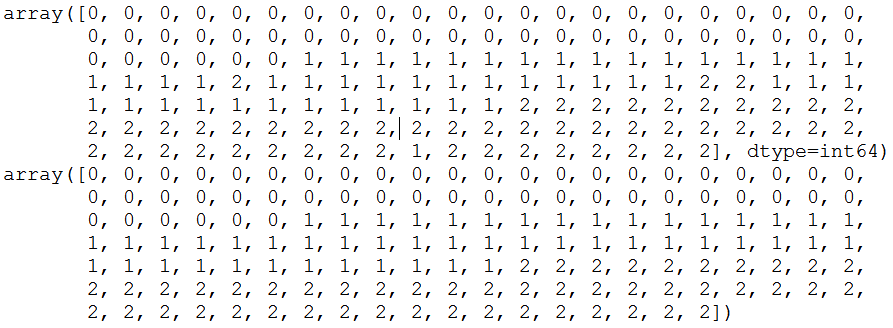
\includegraphics[width=0.5\textwidth]{number_diff.png}
			\caption{label data}
		\end{center}
	\end{figure}
	First array is EM algorithm classification. Second array is answer classification.\\
	Three points are mis-classified.

	\begin{figure}[h]
		\begin{center}
			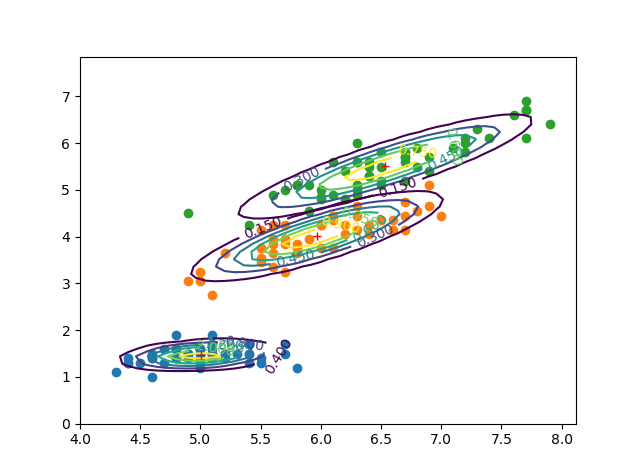
\includegraphics[width=0.5\textwidth]{gauss.png}
			\caption{Three gaussian with scatter data points}
		\end{center}
	\end{figure}

	EM algorithm suceeded to find three gaussian model and classified the data points well.

	\clearpage
	\item For your tests, select the correct number of components (K = 3), but also check the result when you use more or less components. How do you choose your initialization $\theta$0? Does this choice have an influence on the result

	When the number of components is 2, the result is the following figure.
	\begin{figure}[h]
		\begin{center}
			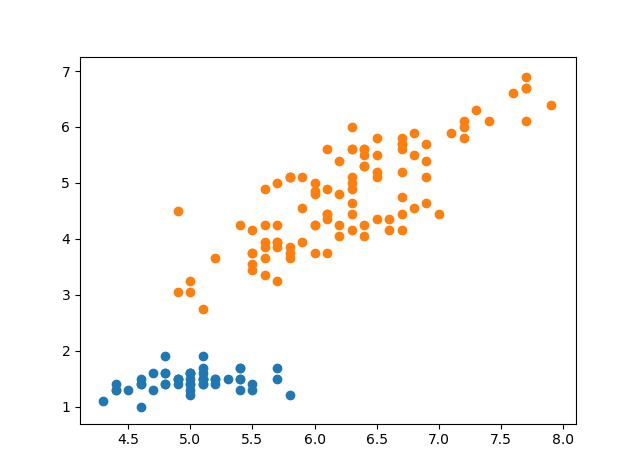
\includegraphics[width=0.4\textwidth]{K2.png}
			\caption{K $=$ 2}
		\end{center}
	\end{figure}

	When the number of components is 4, the result is the following figure.
	\begin{figure}[h]
		\begin{center}
			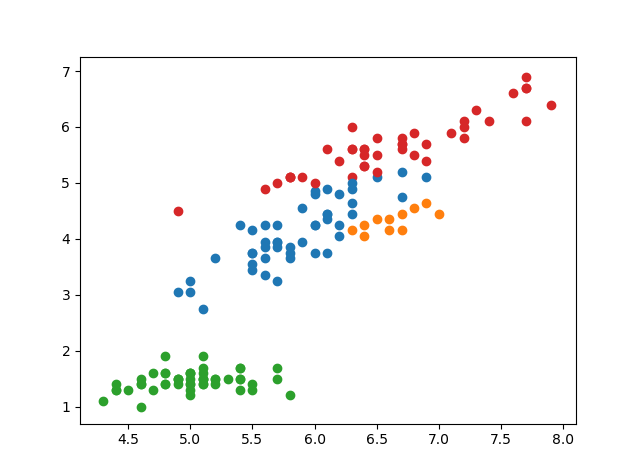
\includegraphics[width=0.4\textwidth]{K4.png}
			\caption{K $=$ 4}
		\end{center}
	\end{figure}

	For initialization $\theta0$, we refered to the class pdf. The following figure is the reference class pdf.

	\begin{figure}[h]
		\begin{center}
			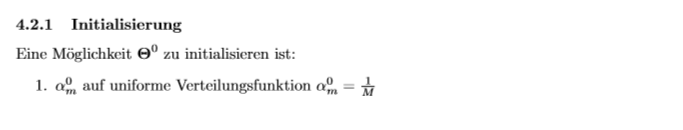
\includegraphics[width=0.5\textwidth]{ref1.png}
			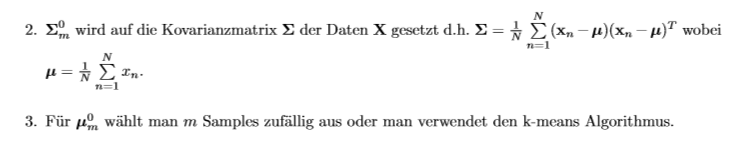
\includegraphics[width=0.5\textwidth]{ref2.png}
			\caption{The initialization process in the class pdf}
		\end{center}
	\end{figure}


	The initialization process influences the EM algorithm result. When the randomly selected points, for calculating mean value, is well chosen, the result is accurate. That is, the result is accurate when the first random selected points are from first answer label group, the second random selected points are from second answer label group and the third random selected points are from third answer label group.

	\clearpage
	\item plot the log-likelihood function over the iterations! What is the behavior of this function over the iterations?

	\begin{figure}[h]
		\begin{center}
			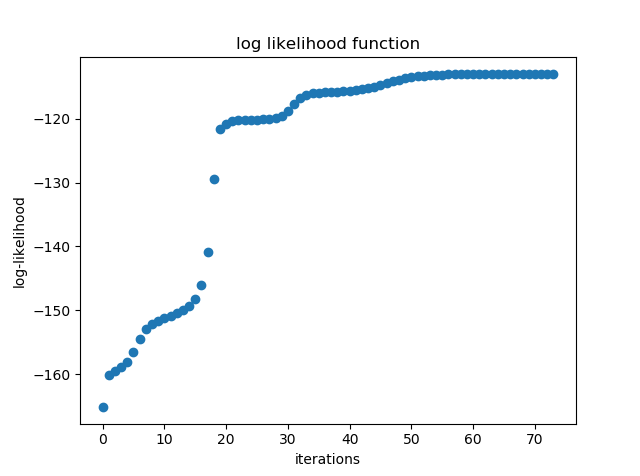
\includegraphics[width=0.5\textwidth]{log_likelihood.png}
			\caption{The log-likelihood function over iterations}
		\end{center}
	\end{figure}
	As shown in Figure 4, the log-likelihood increases over iterations. That is, likelihood increased over iterations. And about 50th iteration, the function looks convering to the value, -112.96270776709655. Therfore, the process stops even though it didn't reach the max iteration number.\\

	\item Make a scatter plot of the data that shows the result of the soft-classification that is done in the E-step

	\begin{figure}[h]
		\begin{center}
			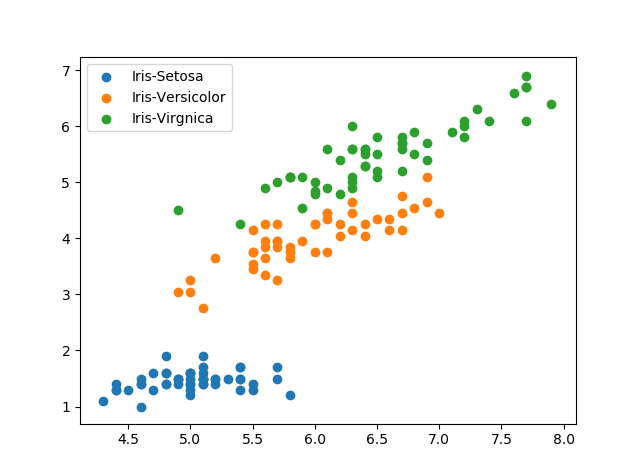
\includegraphics[width=0.3\textwidth]{3class.png}
			\caption{The EM algorithm soft-classification}
			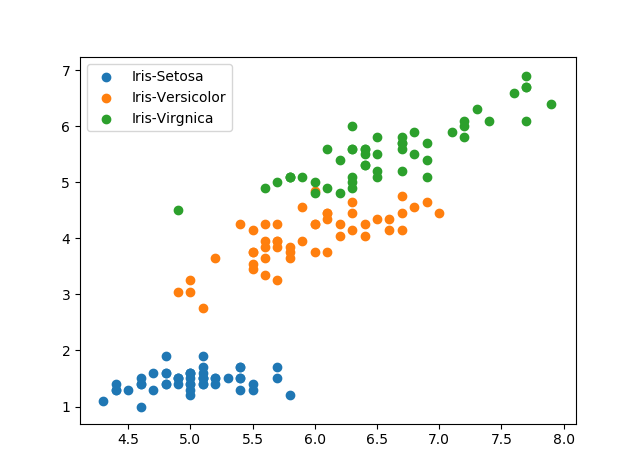
\includegraphics[width=0.3\textwidth]{answer.png}
			\caption{The answer classification}
		\end{center}
	\end{figure}

	The EM algorithm classifies well the points when it is compared with the answer classification. EM algorithm fails to classify the points near the boundary of iris-Versicolor and iris-Virgnica.
	\end{itemize}

	\subsubsection{Perform all of the above-mentioned tasks for the K-means algorithm}
	\subsubsection{You may additionally choose any other pair of features; how would this change the classification accuracy}

	\subsection{4 dimensional feature}
	\subsubsection{EM algorithm tasks}
	\begin{itemize}
		\item Compare the result with the labeled data set (i.e., consider labels as well). Make a scatter plot of the data and plot the Gaussian mixture model over this plot.
		
		\begin{figure}[h]
			\begin{center}
				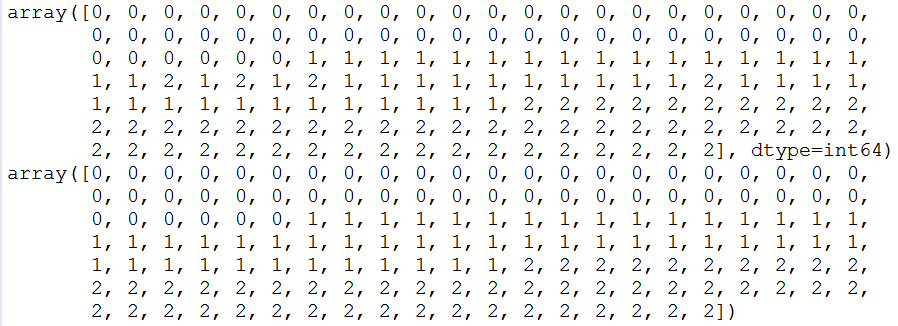
\includegraphics[width=0.5\textwidth]{4_number_diff.png}
				\caption{label data}
			\end{center}
		\end{figure}
		First array is EM algorithm classification. Second array is answer classification.\\
		Four points are mis-classified.
		
		\begin{figure}[h]
			\begin{center}
				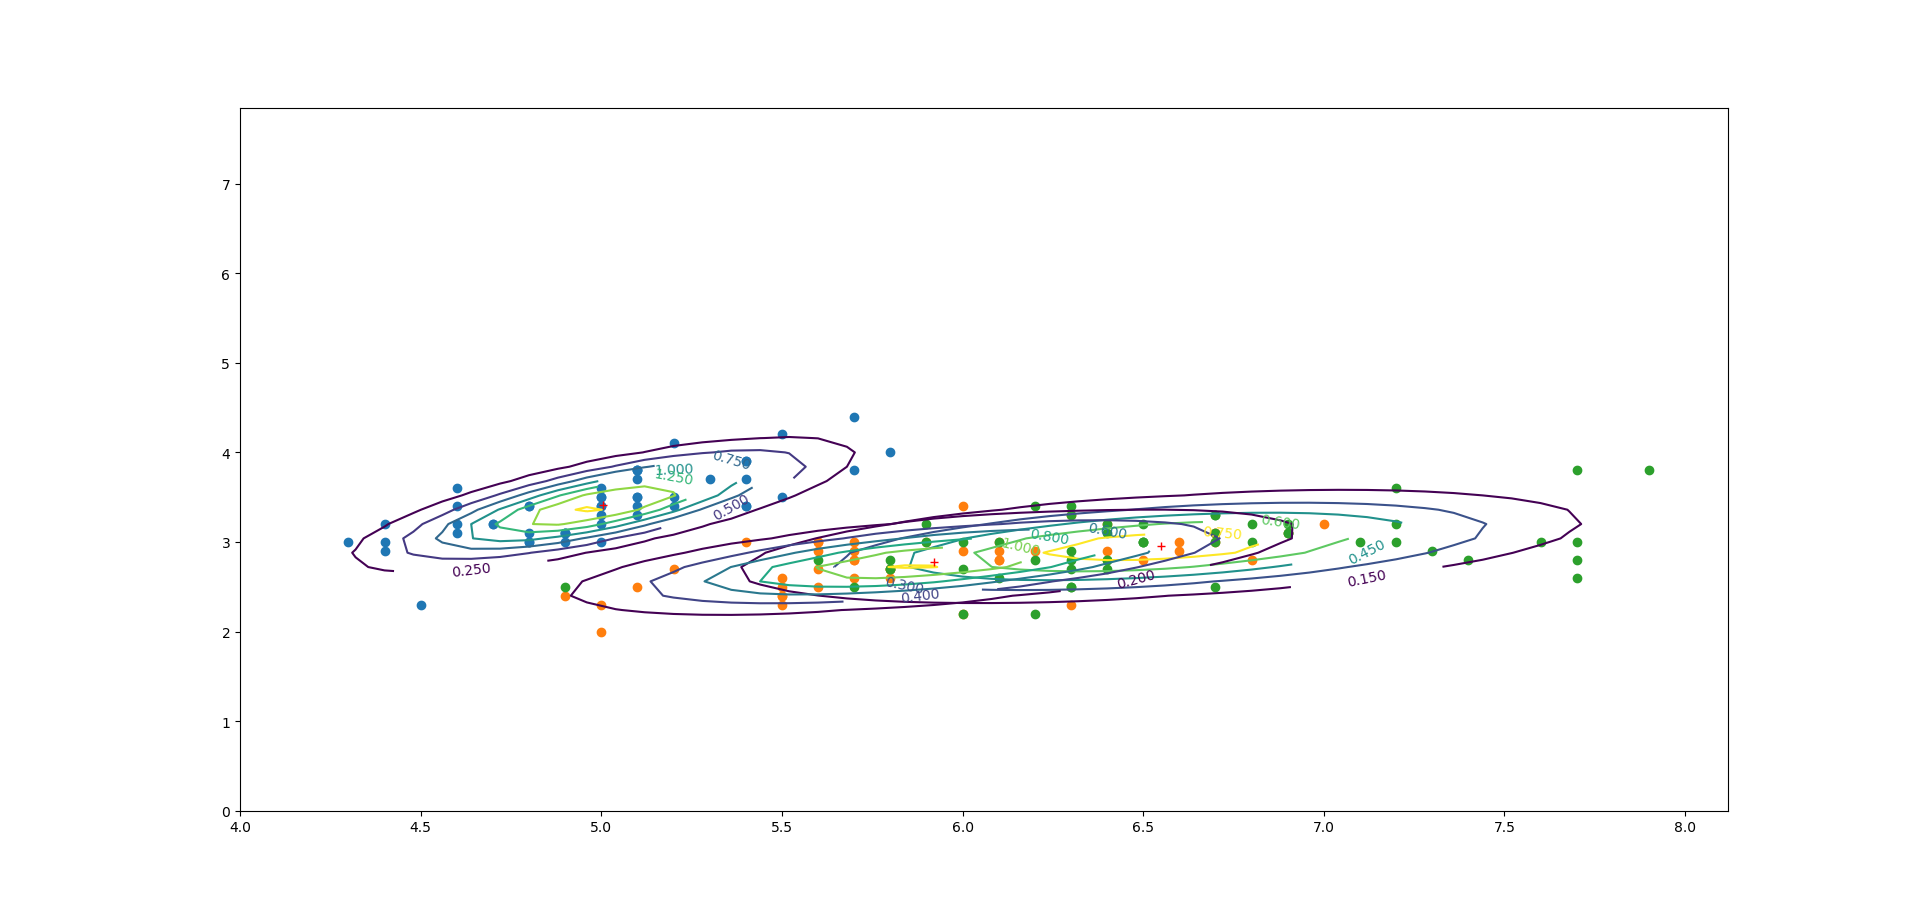
\includegraphics[width=0.5\textwidth]{4_gauss.png}
				\caption{Three gaussian with scatter data points}
			\end{center}
		\end{figure}
		
		EM algorithm suceeded to find three gaussian model and classified the data points well.
		
		\item For your tests, select the correct number of components (K = 3), but also check the result when you use more or less components. How do you choose your initialization $\theta$0? Does this choice have an influence on the result
		When the number of components is 2, the result is the following figure.
		
		\begin{figure}[h]
			\begin{center}
				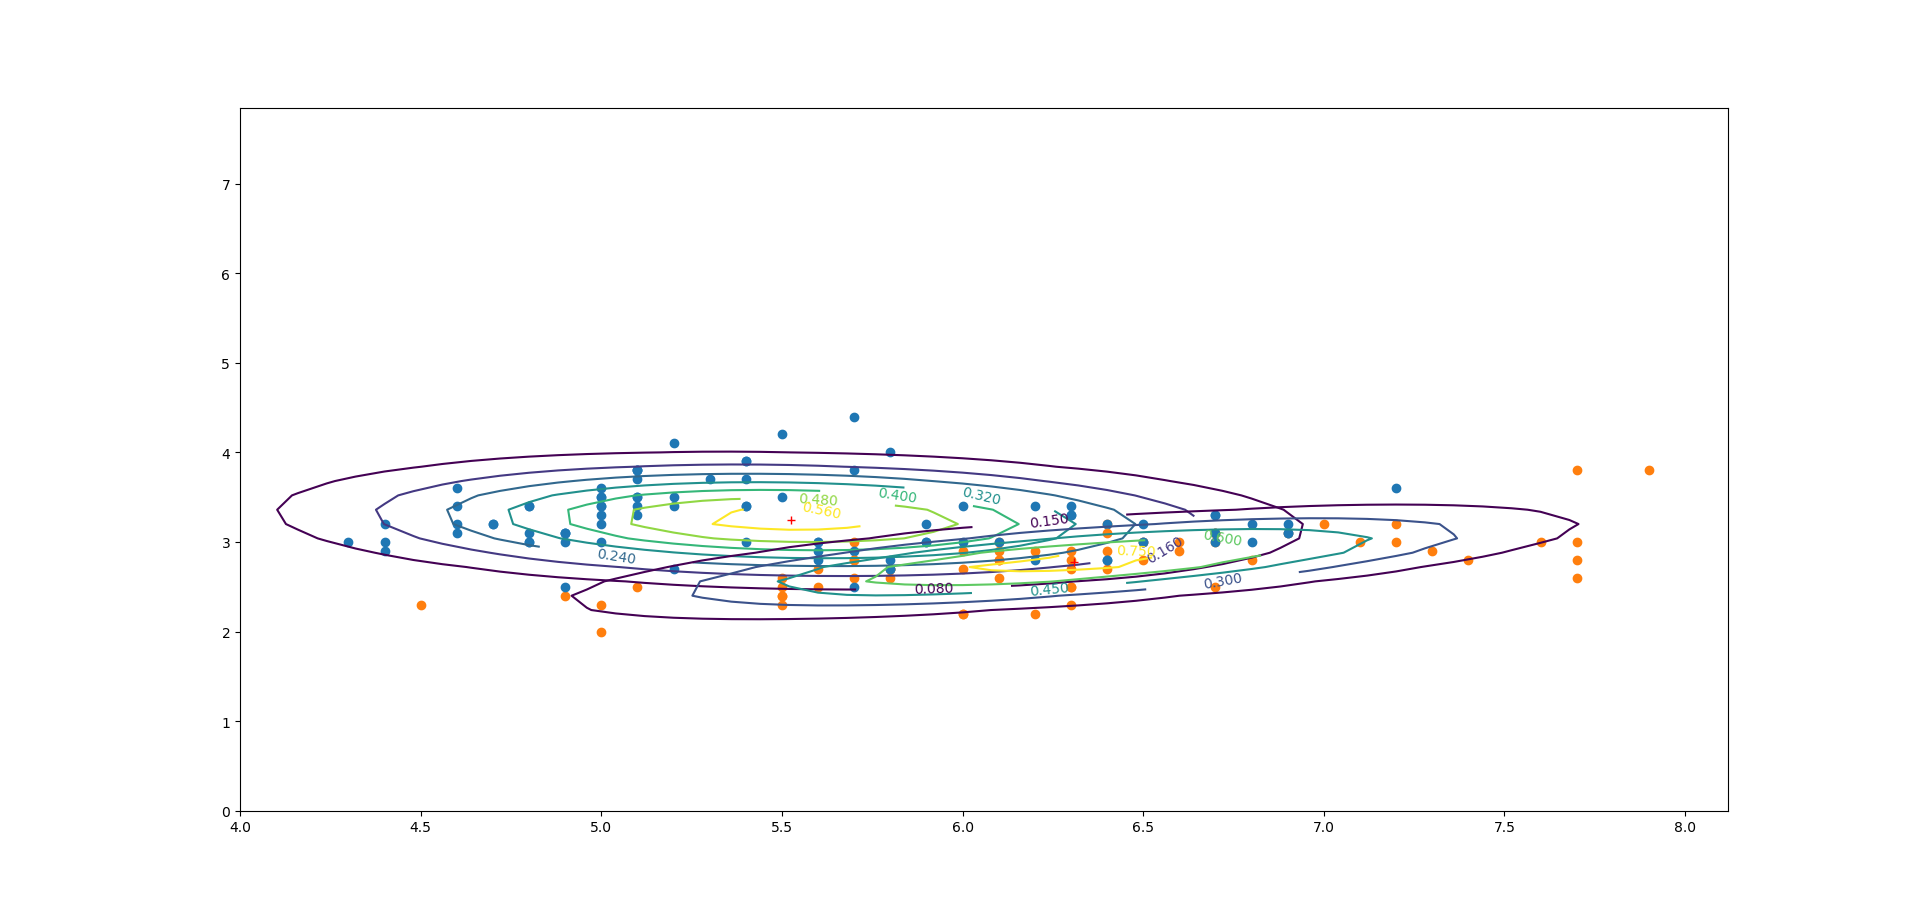
\includegraphics[width=0.4\textwidth]{4_K2.png}
				\caption{K $=$ 2}
			\end{center}
		\end{figure}
		
		\clearpage
		When the number of components is 4, the result is the following figure.
		\begin{figure}[h]
			\begin{center}
				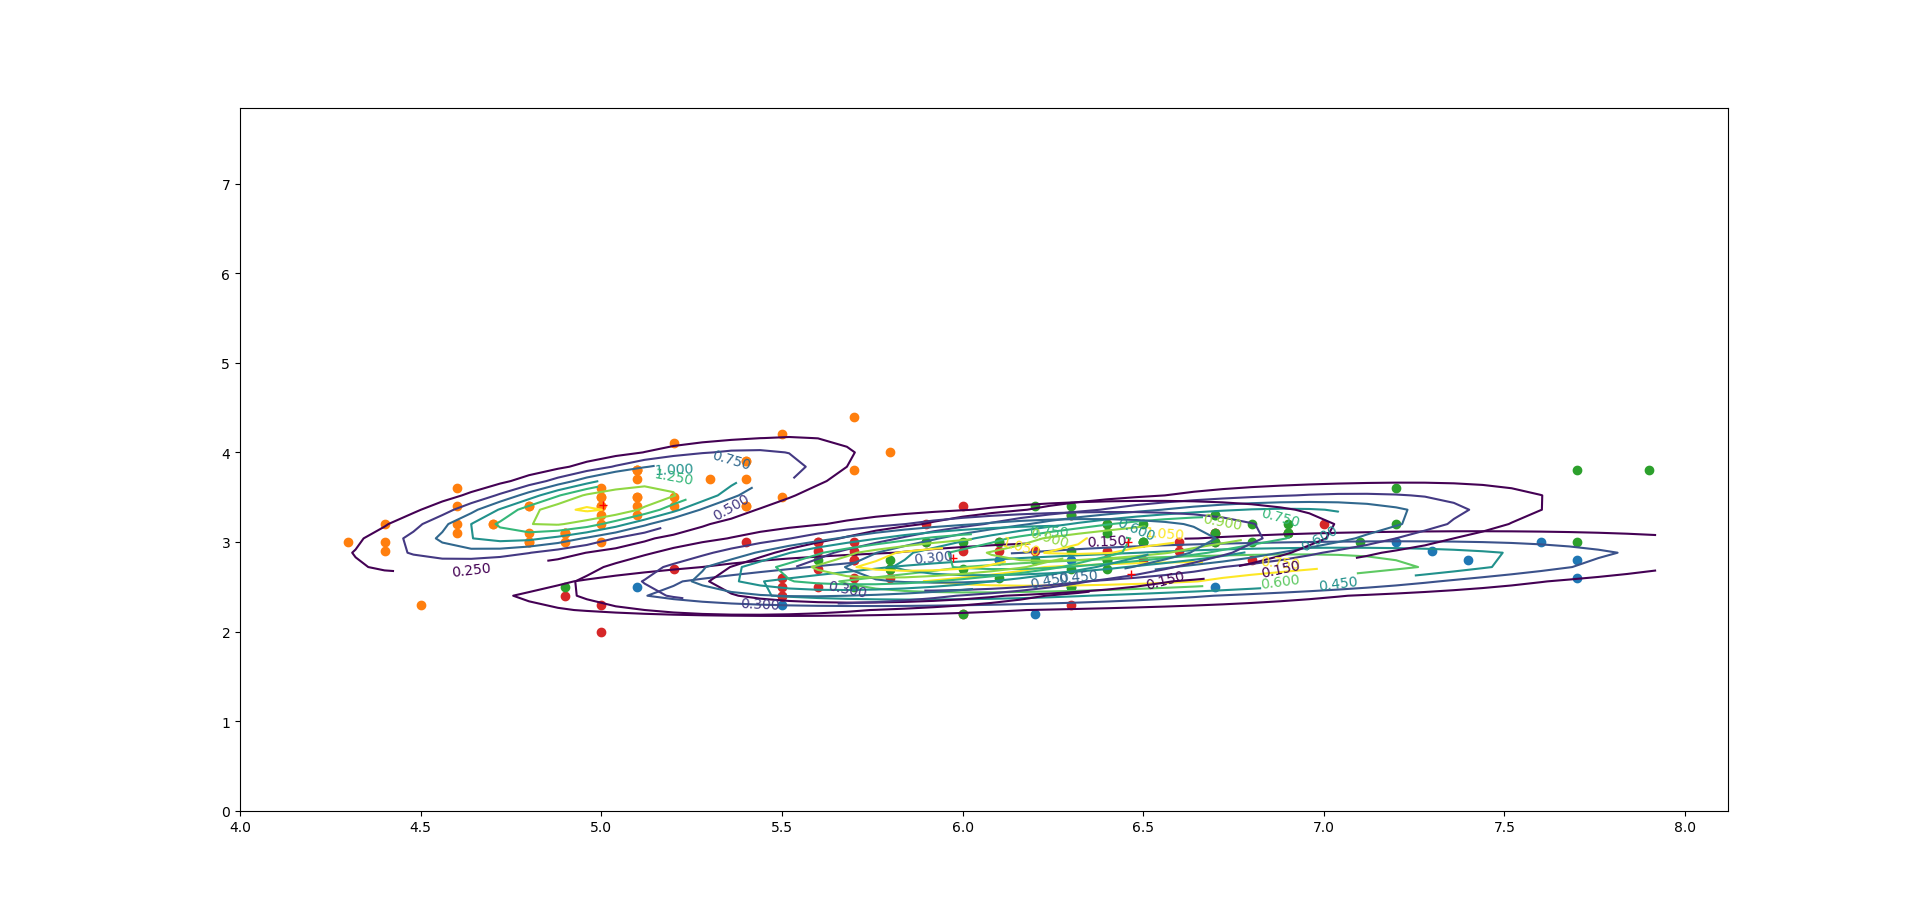
\includegraphics[width=0.4\textwidth]{4_K4.png}
				\caption{K $=$ 4}
			\end{center}
		\end{figure}
		
		Initalizaiton $\theta$0 is the same with the dimension 2.\\
		As written in section 1.1.1, the initialization process affects the result.
		
		\item plot the log-likelihood function over the iterations! What is the behavior of this function over the iterations?
		
		\begin{figure}[h]
			\begin{center}
				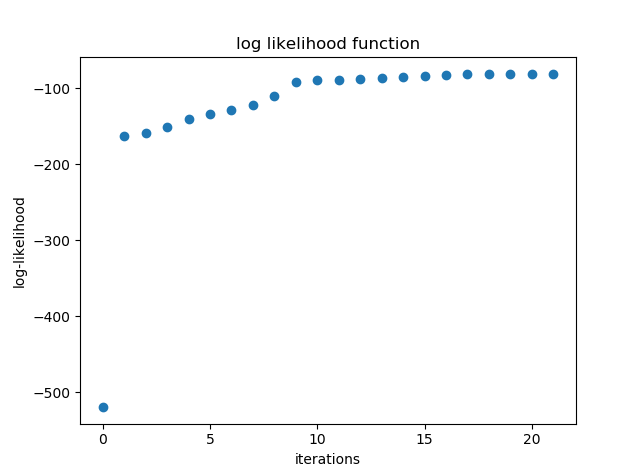
\includegraphics[width=0.4\textwidth]{4_log_likelihood.png}
				\caption{The log-likelihood function over iterations}
			\end{center}
		\end{figure}
		As shown in Figure 4, the log-likelihood increases over iterations. That is, likelihood increased over iterations. And about 25th iteration, the function looks convering to the value, -87.41158191236445.. Therfore, the process stops even though it didn't reach the max iteration number.\\
		
		\clearpage
		\item Make a scatter plot of the data that shows the result of the soft-classification that is done in the E-step
		
		\begin{figure}[h]
			\begin{center}
				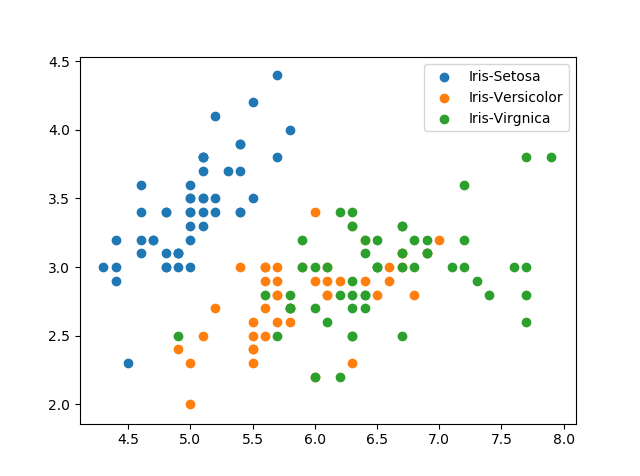
\includegraphics[width=0.3\textwidth]{4class.png}
				\caption{The EM algorithm soft-classification}
				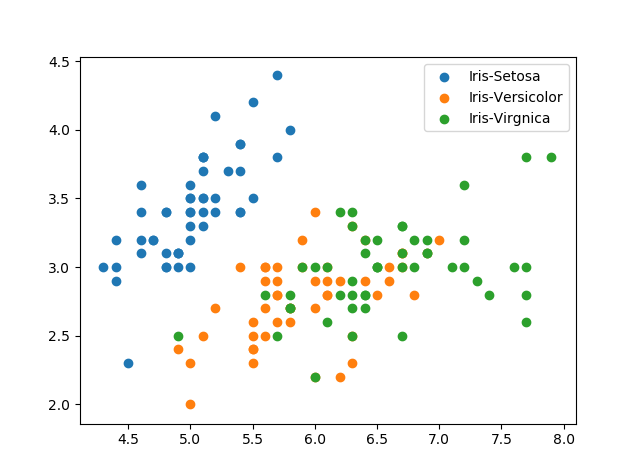
\includegraphics[width=0.3\textwidth]{4_answer.png}
				\caption{The answer classification}
			\end{center}
		\end{figure}
		
		The EM algorithm classifies well the points when it is compared with the answer classification. EM algorithm fails to classify the points near the boundary of iris-Versicolor and iris-Virgnica.
		
	\end{itemize}
	\subsubsection{How do the convergence properties and the accuracy of you classification change in comparison to scenario 2.1? }
	\begin{itemize}
		\item EM-algorithm \\
		The convergence value of log likelihood function increased. In the scenario 2.1, the value was -112.96. However, in the scenario 2.2, the value increased to -87.41. Also, the total iteration decreased in the scenario 2.2. The value decreased from 75 to 26.\\
		Also, we compared the scenario 2.1 and 2.2 with each 10 trials. Overall, the EM classifies the data points better in 2.2 scenario. The accuarcy of 2.2 scenario is higher than that of 2.1 scenario. Because the EM algorithm in 2.2 scenario has more additional information about the dataset.
		 
	\end{itemize}
	
	\subsubsection{Within your EM-function confine the structure of the covariance matrices to diagonal matrices! What is the influence on the result.}
        \clearpage
	\subsection{Processing the data with PCA }
	\subsubsection{How much of the variance in the data is explained this way?}
        \begin{itemize}
          \item original variance(sum of eigenvalues) -  4.499157046979866
          \item associated eigenvalues - 4.15886089, 0.23573307
          \item the amount of explained variance - 0.9767594057574307
        \end{itemize}
        \subsubsection{How does the performance of your algorithms compare to scenario 2.1 and scenario 2.2?}

          Scenario 2.1 has no difference at performance for both algorithms. Actually it takes more time to do PCA.
          The amount of explained variance is 1. The data from PCA is rotated original data that eigenvectors are the axes.

          \begin{figure}[h!]
            \centering
            \begin{minipage}[t]{6.5cm}
              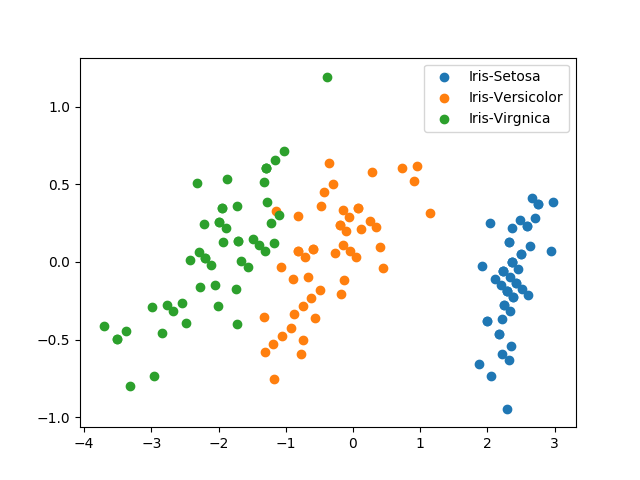
\includegraphics[width=1.0\textwidth]{pca_em_1_ans.png}
              \caption{answer for pca scenario 1}
            \end{minipage}
            \hspace{2cm}
            \begin{minipage}[t]{6.5cm}
              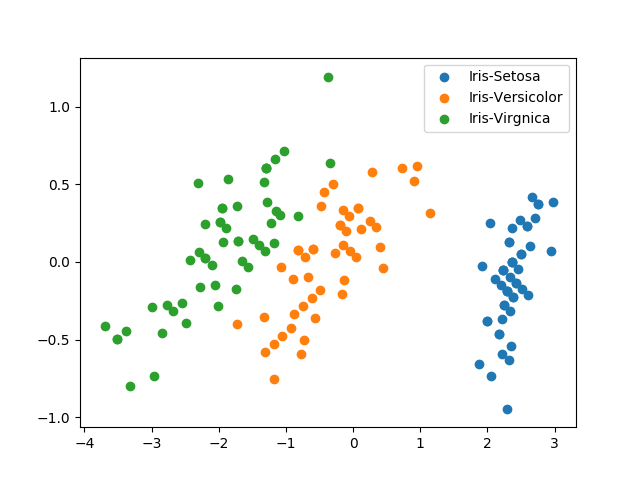
\includegraphics[width=1.0\textwidth]{pca_em_1_1.png}
              \caption{scatter plot for scenario 1. EM}
            \end{minipage}
            \begin{minipage}[t]{6.5cm}
              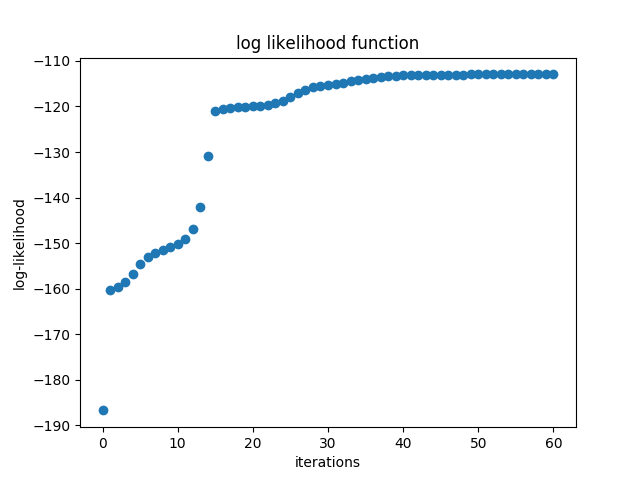
\includegraphics[width=1.0\textwidth]{pca_em_1_2.png}
              \caption{log-likelihood plot for scenario 1. EM}
            \end{minipage}
            \hspace{2cm}
            \begin{minipage}[t]{6.5cm}
              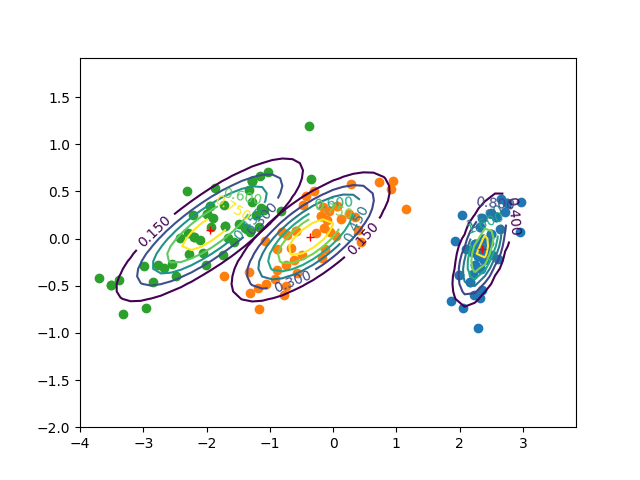
\includegraphics[width=1.0\textwidth]{pca_em_1_3.png}
              \caption{scatter plot with Gaussian for scenario 1. EM}
            \end{minipage}
            \begin{minipage}[t]{6.5cm}
              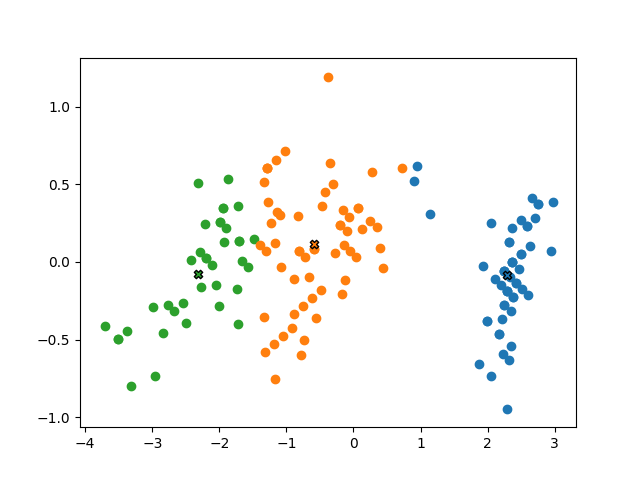
\includegraphics[width=1.0\textwidth]{pca_k_1_1.png}
              \caption{scatter plot for scenario 1. K-means}
            \end{minipage}
            \hspace{2cm}
            \begin{minipage}[t]{6.5cm}
              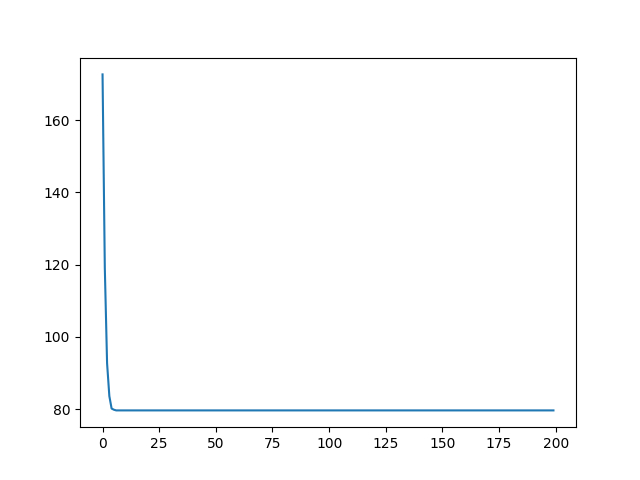
\includegraphics[width=1.0\textwidth]{pca_k_1_2.png}
              \caption{cumulative distance for k-means plot for scenario 1. K-means}
            \end{minipage}
          \end{figure}

        EM showed better performance in scenario 2.2. PCA reduced the dimension of data to 2 so it took less time and showed more accuracy.

        \begin{figure}[h!]
            \centering
            \begin{minipage}[t]{6.5cm}
              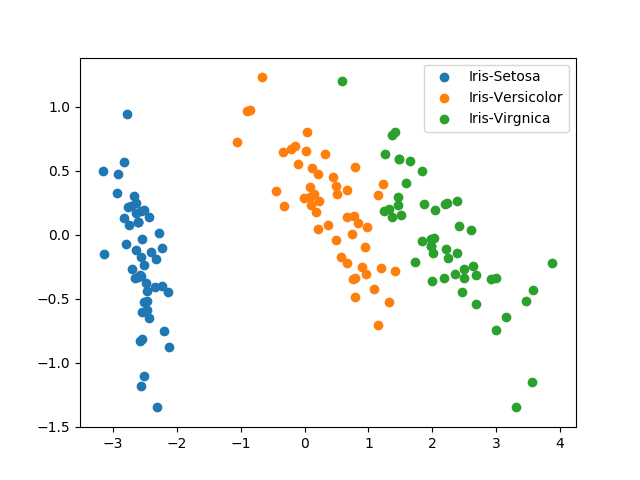
\includegraphics[width=1.0\textwidth]{pca_em_2_ans.png}
              \caption{answer for pca scenario 2}
            \end{minipage}
            \hspace{2cm}
            \begin{minipage}[t]{6.5cm}
              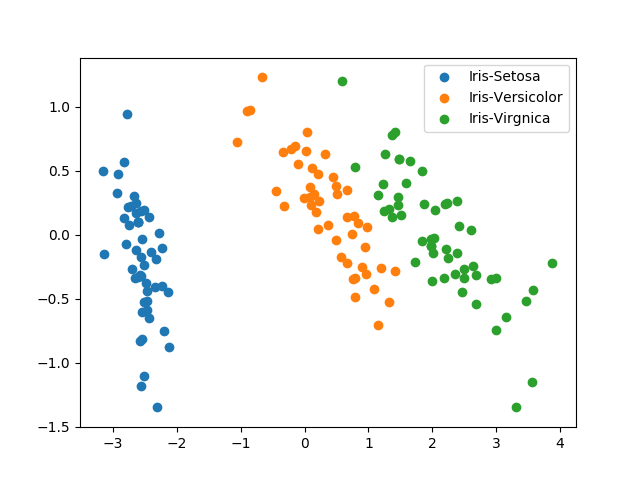
\includegraphics[width=1.0\textwidth]{pca_em_2_1.png}
              \caption{scatter plot for scenario 2. EM}
            \end{minipage}
            \begin{minipage}[t]{6.5cm}
              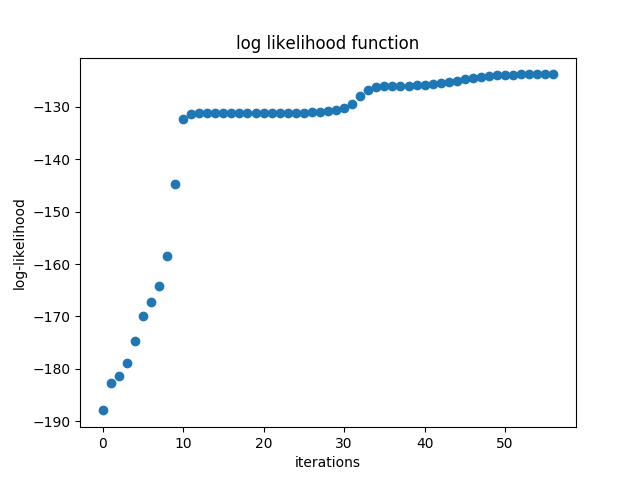
\includegraphics[width=1.0\textwidth]{pca_em_2_2.png}
              \caption{log-likelihood plot for scenario 2. EM}
            \end{minipage}
            \hspace{2cm}
            \begin{minipage}[t]{6.5cm}
              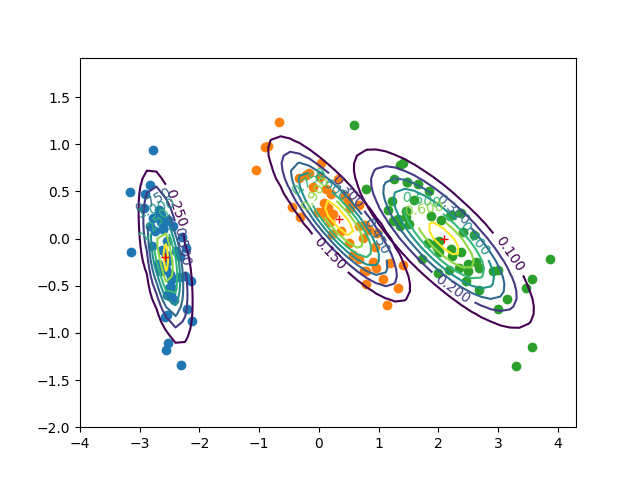
\includegraphics[width=1.0\textwidth]{pca_em_2_3.png}
              \caption{scatter plot with Gaussian for scenario 2. EM}
            \end{minipage}
            \begin{minipage}[t]{6.5cm}
              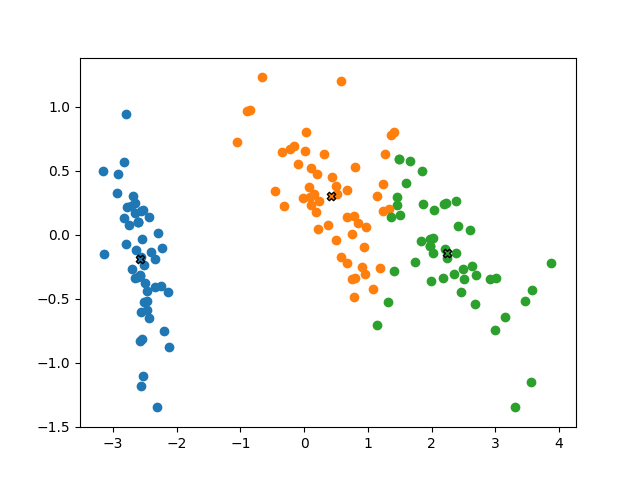
\includegraphics[width=1.0\textwidth]{pca_k_2_1.png}
              \caption{scatter plot for scenario 2. K-means}
            \end{minipage}
            \hspace{2cm}
            \begin{minipage}[t]{6.5cm}
              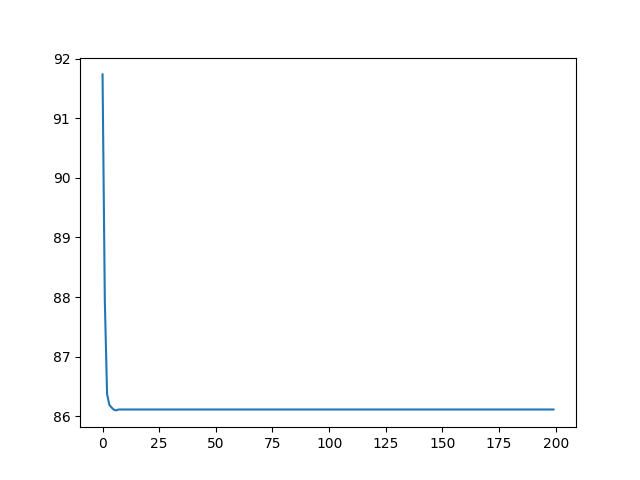
\includegraphics[width=1.0\textwidth]{pca_k_2_2.png}
              \caption{cumulative distance for k-means plot for scenario 2. K-means}
            \end{minipage}
        \end{figure}
        \clearpage
	\subsubsection{Apply PCA with whitening, so that the transformed data has zero mean and a unit covariance matrix. How does this influence the choice of your initialization?}

        \clearpage
	\section{Samples from a Gaussian Mixture Model}
	\subsection{Write a function Y = sample-GMM(alpha, mu, cov, N)}
	\subsection{Using a GMM of your choice$ (K > 3)$, demonstrate the correctness of your function}
\end{document}
